\documentclass[a4paper]{article}
\usepackage[top=1.7cm, bottom=2.5cm, left=1.7cm, right=1.7cm]{geometry}
\usepackage{parskip}
\usepackage{graphicx}
\usepackage{amsmath}
\usepackage{amsfonts}
\usepackage{amssymb}
\usepackage{hyperref}
\usepackage{listings}
\usepackage{epsf} 
\usepackage{float}

\title{MA3505 Multivariate Statistics Project 1}
\date{\today}

\begin{document}
\maketitle


\section{Introduction and exploratory data analysis for the variables.}


\section{Analysis to answer each research question}

\subsection{Question 1}


\subsection{Question 2}


\subsection{Question 3}

\subsubsection{Cleveland}

From running variance inflation factor we get the following

\lstinputlisting[frame=single]{question3output/clevif.txt}

Here we see the variables, ekgmo, ekgyr, cmo and cyr are collinear with other variables in the model. 


\begin{figure}[H]
	\begin{center}
		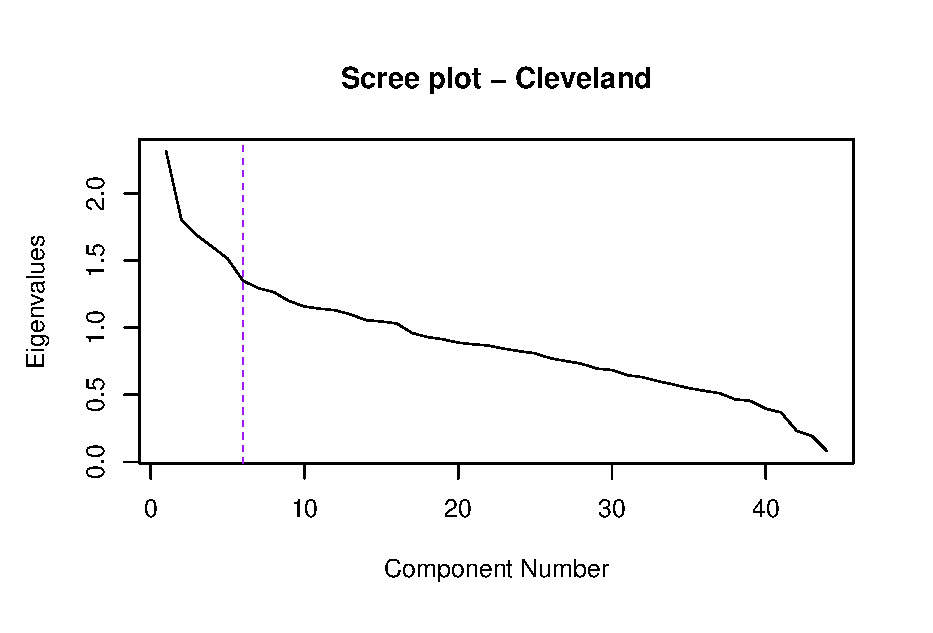
\includegraphics[width=12cm]{question3output/clescreeplot.eps} 
	\end{center}
	\caption{Scree plot for PCA of Cleveland}
	\label{q3-cle-screeplot}
\end{figure}

From the scree plot in Figure \ref{q3-cle-screeplot} we see that we keep 6 components.

We have the loadings of each components as follows. 

\lstinputlisting[frame=single]{question3output/clepcaloadings.txt}

\subsubsection{Hungary}

\begin{figure}[H]
	\begin{center}
		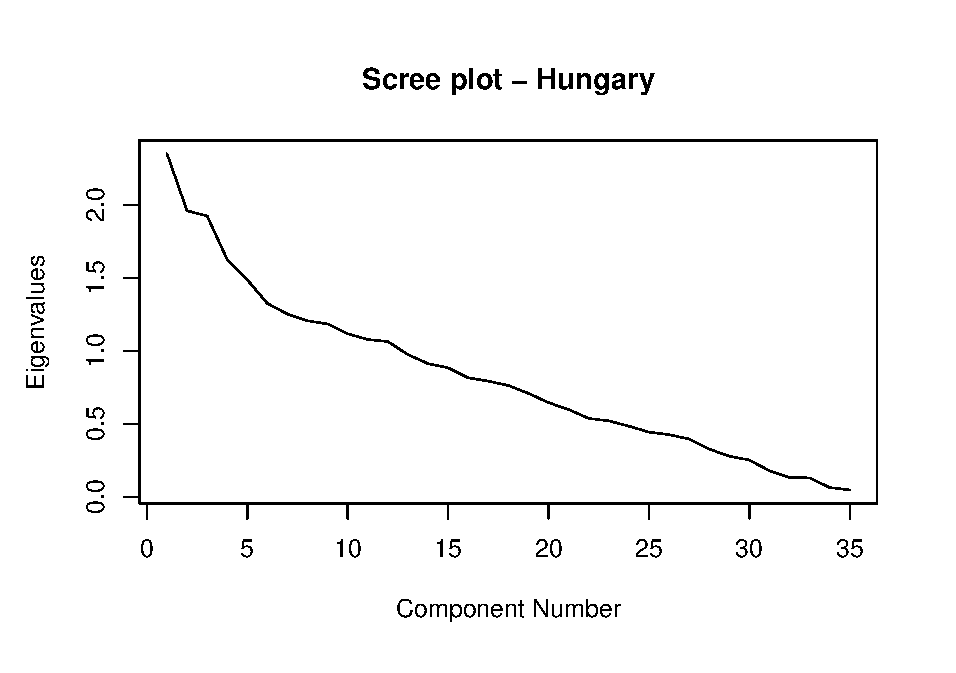
\includegraphics[width=12cm]{question3output/hunscreeplot.eps} 
	\end{center}
	\caption{Scree plot for PCA of Hungary}
	\label{q3-hun-screeplot}
\end{figure}

From the scree plot in Figure \ref{q3-hun-screeplot} we see that we keep 6 components.

We have the loadings of each components as follows. 

\lstinputlisting[frame=single]{question3output/hunpcaloadings.txt}

\subsubsection{Longbeach}

\begin{figure}[H]
	\begin{center}
		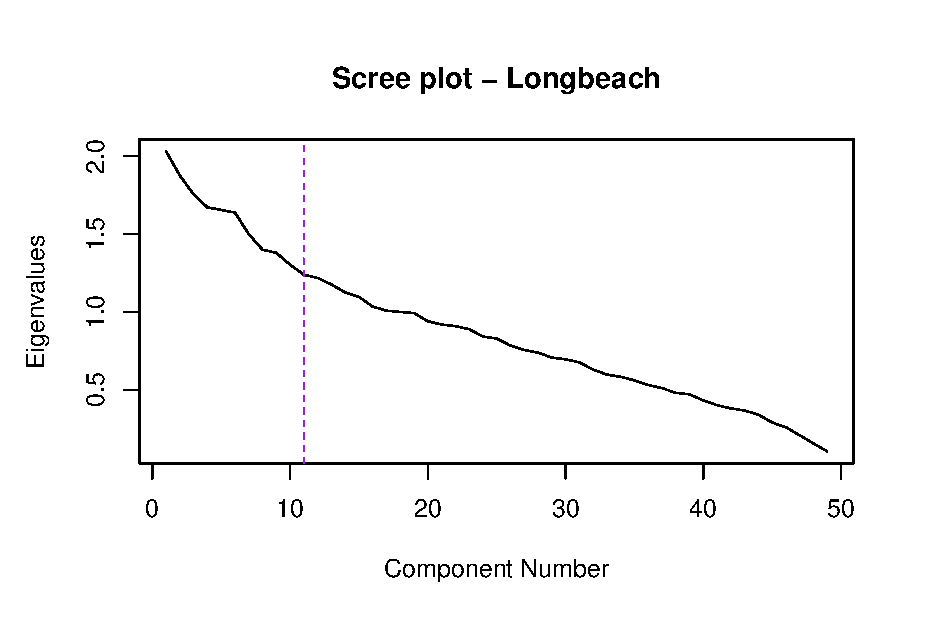
\includegraphics[width=12cm]{question3output/lonscreeplot.eps} 
	\end{center}
	\caption{Scree plot for PCA of Longbeach}
	\label{q3-lon-screeplot}
\end{figure}

From the scree plot in Figure \ref{q3-lon-screeplot} we see that we keep 11 components.

We have the loadings of each components as follows. 

\lstinputlisting[frame=single]{question3output/lonpcaloadings.txt}

\subsubsection{Switzerland}

\begin{figure}[H]
	\begin{center}
		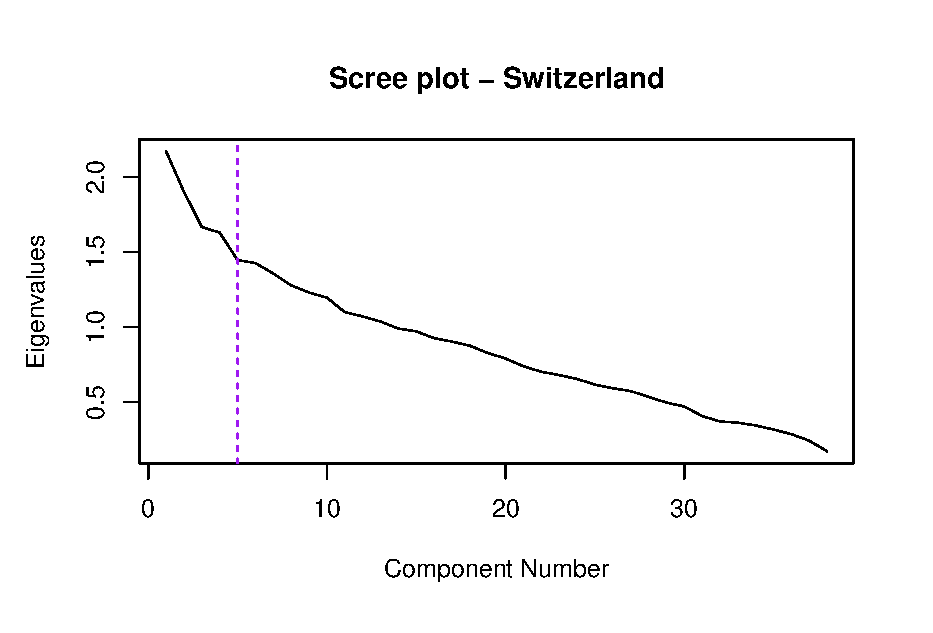
\includegraphics[width=12cm]{question3output/swiscreeplot.eps} 
	\end{center}
	\caption{Scree plot for PCA of Switzerland}
	\label{q3-swi-screeplot}
\end{figure}

From the scree plot in Figure \ref{q3-swi-screeplot} we see that we keep 5 components.

We have the loadings of each components as follows. 

\lstinputlisting[frame=single]{question3output/swipcaloadings.txt}

\subsection{Question 4}

\section{Summary}

\end{document}
